\section{dg::Ray\-Tracer Class Reference}
\label{classdg_1_1RayTracer}\index{dg::RayTracer@{dg::RayTracer}}
{\tt \#include $<$Ray\-Tracer.h$>$}

Collaboration diagram for dg::Ray\-Tracer:\begin{figure}[H]
\begin{center}
\leavevmode
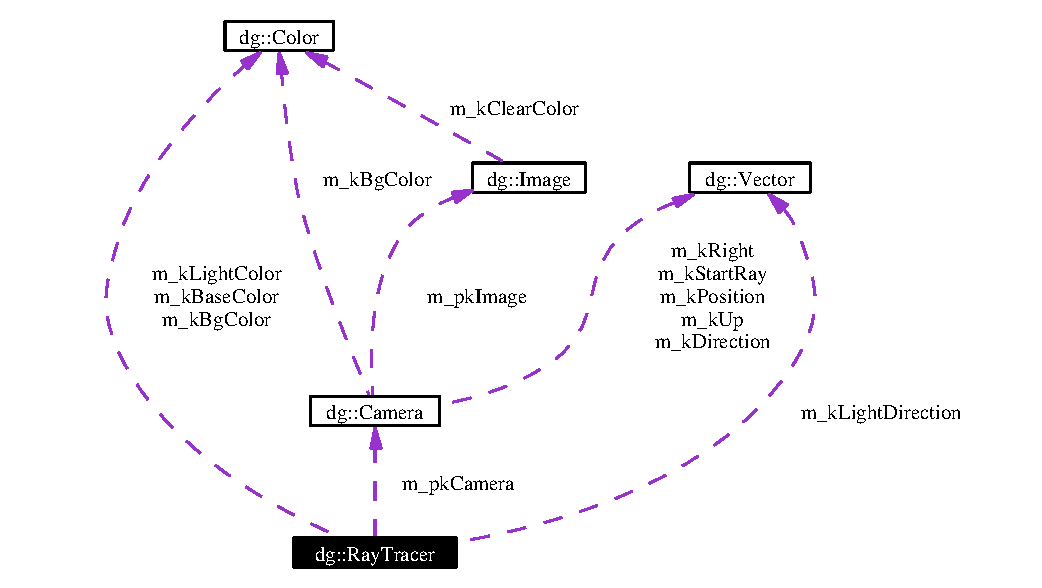
\includegraphics[width=267pt]{classdg_1_1RayTracer__coll__graph}
\end{center}
\end{figure}
\subsection*{Public Types}
\begin{CompactItemize}
\item 
typedef {\bf Real}($\ast$ {\bf Function} )({\bf Real} f\-X, {\bf Real} f\-Y, {\bf Real} f\-Z)
\end{CompactItemize}
\subsection*{Public Methods}
\begin{CompactItemize}
\item 
{\bf Ray\-Tracer} ({\bf Function} pv\-Function=NULL, {\bf Camera} $\ast$pk\-Camera=NULL)
\item 
{\bf $\sim$Ray\-Tracer} ()
\item 
void {\bf set\-Camera} ({\bf Camera} $\ast$pk\-Camera)
\item 
const {\bf Camera} $\ast$ {\bf get\-Camera} () const
\item 
void {\bf set\-Function} ({\bf Function} pv\-Function)
\item 
{\bf Vector} {\bf get\-Light\-Direction} () const
\item 
void {\bf set\-Light\-Direction} (const {\bf Vector} \&rk\-Light)
\item 
{\bf Color} {\bf get\-Light\-Color} () const
\item 
void {\bf set\-Light\-Color} (const {\bf Color} \&rk\-Light)
\item 
void {\bf set\-Normal\-Epsilon} ({\bf Real} f\-Epsilon)
\item 
{\bf Real} {\bf get\-Normal\-Epsilon} () const
\item 
void {\bf set\-Ray\-Epsilon} ({\bf Real} f\-Epsilon)
\item 
{\bf Real} {\bf get\-Ray\-Epsilon} () const
\item 
void {\bf set\-Iso\-Level} ({\bf Real} f\-Level)
\item 
{\bf Real} {\bf get\-Iso\-Level} () const
\item 
void {\bf set\-Samples} ({\bf UInt} ui\-Samples)
\item 
{\bf UInt} {\bf get\-Samples} () const
\item 
{\bf UInt} {\bf get\-Ray\-Hits} () const
\item 
void {\bf set\-Blur} (bool b\-Blur)
\item 
bool {\bf get\-Blur} () const
\item 
void {\bf set\-Background} (const {\bf Color} \&rk\-Color)
\item 
{\bf Color} {\bf get\-Background} () const
\item 
{\bf Real} {\bf get\-Ambient} () const
\item 
void {\bf set\-Ambient} ({\bf Real} f\-Ambient)
\item 
{\bf Real} {\bf get\-Diffuse} () const
\item 
void {\bf set\-Diffuse} ({\bf Real} f\-Diffuse)
\item 
{\bf Real} {\bf get\-Specular} () const
\item 
void {\bf set\-Specular} ({\bf Real} f\-Specular)
\item 
{\bf Real} {\bf get\-Roughness} () const
\item 
void {\bf set\-Roughness} ({\bf Real} f\-Roughness)
\item 
{\bf Color} {\bf get\-Base\-Color} () const
\item 
void {\bf set\-Base\-Color} (const {\bf Color} \&rk\-Base)
\item 
void {\bf render} ()
\item 
void {\bf render} ({\bf UInt} ui\-Start\-Line, {\bf UInt} ui\-End\-Line)
\end{CompactItemize}


\subsection{Member Typedef Documentation}
\index{dg::RayTracer@{dg::Ray\-Tracer}!Function@{Function}}
\index{Function@{Function}!dg::RayTracer@{dg::Ray\-Tracer}}
\subsubsection{\setlength{\rightskip}{0pt plus 5cm}typedef {\bf Real}($\ast$ dg::Ray\-Tracer::Function)({\bf Real} f\-X, {\bf Real} f\-Y, {\bf Real} f\-Z)}\label{classdg_1_1RayTracer_s0}




Definition at line 18 of file Ray\-Tracer.h.

\subsection{Constructor \& Destructor Documentation}
\index{dg::RayTracer@{dg::Ray\-Tracer}!RayTracer@{RayTracer}}
\index{RayTracer@{RayTracer}!dg::RayTracer@{dg::Ray\-Tracer}}
\subsubsection{\setlength{\rightskip}{0pt plus 5cm}Ray\-Tracer::Ray\-Tracer ({\bf Function} {\em pv\-Function} = NULL, {\bf Camera} $\ast$ {\em pk\-Camera} = NULL)}\label{classdg_1_1RayTracer_a0}




Definition at line 8 of file Ray\-Tracer.cpp.\index{dg::RayTracer@{dg::Ray\-Tracer}!~RayTracer@{$\sim$RayTracer}}
\index{~RayTracer@{$\sim$RayTracer}!dg::RayTracer@{dg::Ray\-Tracer}}
\subsubsection{\setlength{\rightskip}{0pt plus 5cm}Ray\-Tracer::$\sim$Ray\-Tracer ()}\label{classdg_1_1RayTracer_a1}




Definition at line 26 of file Ray\-Tracer.cpp.

\subsection{Member Function Documentation}
\index{dg::RayTracer@{dg::Ray\-Tracer}!getAmbient@{getAmbient}}
\index{getAmbient@{getAmbient}!dg::RayTracer@{dg::Ray\-Tracer}}
\subsubsection{\setlength{\rightskip}{0pt plus 5cm}{\bf Real} dg::Ray\-Tracer::get\-Ambient ()\hspace{0.3cm}{\tt  [inline]}}\label{classdg_1_1RayTracer_a22}




Definition at line 259 of file Ray\-Tracer.h.\index{dg::RayTracer@{dg::Ray\-Tracer}!getBackground@{getBackground}}
\index{getBackground@{getBackground}!dg::RayTracer@{dg::Ray\-Tracer}}
\subsubsection{\setlength{\rightskip}{0pt plus 5cm}{\bf Color} dg::Ray\-Tracer::get\-Background ()\hspace{0.3cm}{\tt  [inline]}}\label{classdg_1_1RayTracer_a21}




Definition at line 231 of file Ray\-Tracer.h.\index{dg::RayTracer@{dg::Ray\-Tracer}!getBaseColor@{getBaseColor}}
\index{getBaseColor@{getBaseColor}!dg::RayTracer@{dg::Ray\-Tracer}}
\subsubsection{\setlength{\rightskip}{0pt plus 5cm}{\bf Color} dg::Ray\-Tracer::get\-Base\-Color ()\hspace{0.3cm}{\tt  [inline]}}\label{classdg_1_1RayTracer_a30}




Definition at line 221 of file Ray\-Tracer.h.\index{dg::RayTracer@{dg::Ray\-Tracer}!getBlur@{getBlur}}
\index{getBlur@{getBlur}!dg::RayTracer@{dg::Ray\-Tracer}}
\subsubsection{\setlength{\rightskip}{0pt plus 5cm}bool dg::Ray\-Tracer::get\-Blur ()\hspace{0.3cm}{\tt  [inline]}}\label{classdg_1_1RayTracer_a19}




Definition at line 211 of file Ray\-Tracer.h.\index{dg::RayTracer@{dg::Ray\-Tracer}!getCamera@{getCamera}}
\index{getCamera@{getCamera}!dg::RayTracer@{dg::Ray\-Tracer}}
\subsubsection{\setlength{\rightskip}{0pt plus 5cm}const {\bf Camera} $\ast$ dg::Ray\-Tracer::get\-Camera ()\hspace{0.3cm}{\tt  [inline]}}\label{classdg_1_1RayTracer_a3}




Definition at line 241 of file Ray\-Tracer.h.\index{dg::RayTracer@{dg::Ray\-Tracer}!getDiffuse@{getDiffuse}}
\index{getDiffuse@{getDiffuse}!dg::RayTracer@{dg::Ray\-Tracer}}
\subsubsection{\setlength{\rightskip}{0pt plus 5cm}{\bf Real} dg::Ray\-Tracer::get\-Diffuse ()\hspace{0.3cm}{\tt  [inline]}}\label{classdg_1_1RayTracer_a24}




Definition at line 269 of file Ray\-Tracer.h.\index{dg::RayTracer@{dg::Ray\-Tracer}!getIsoLevel@{getIsoLevel}}
\index{getIsoLevel@{getIsoLevel}!dg::RayTracer@{dg::Ray\-Tracer}}
\subsubsection{\setlength{\rightskip}{0pt plus 5cm}{\bf Real} dg::Ray\-Tracer::get\-Iso\-Level ()\hspace{0.3cm}{\tt  [inline]}}\label{classdg_1_1RayTracer_a14}




Definition at line 181 of file Ray\-Tracer.h.\index{dg::RayTracer@{dg::Ray\-Tracer}!getLightColor@{getLightColor}}
\index{getLightColor@{getLightColor}!dg::RayTracer@{dg::Ray\-Tracer}}
\subsubsection{\setlength{\rightskip}{0pt plus 5cm}{\bf Color} dg::Ray\-Tracer::get\-Light\-Color ()\hspace{0.3cm}{\tt  [inline]}}\label{classdg_1_1RayTracer_a7}




Definition at line 156 of file Ray\-Tracer.h.\index{dg::RayTracer@{dg::Ray\-Tracer}!getLightDirection@{getLightDirection}}
\index{getLightDirection@{getLightDirection}!dg::RayTracer@{dg::Ray\-Tracer}}
\subsubsection{\setlength{\rightskip}{0pt plus 5cm}{\bf Vector} dg::Ray\-Tracer::get\-Light\-Direction ()\hspace{0.3cm}{\tt  [inline]}}\label{classdg_1_1RayTracer_a5}




Definition at line 141 of file Ray\-Tracer.h.\index{dg::RayTracer@{dg::Ray\-Tracer}!getNormalEpsilon@{getNormalEpsilon}}
\index{getNormalEpsilon@{getNormalEpsilon}!dg::RayTracer@{dg::Ray\-Tracer}}
\subsubsection{\setlength{\rightskip}{0pt plus 5cm}{\bf Real} dg::Ray\-Tracer::get\-Normal\-Epsilon ()\hspace{0.3cm}{\tt  [inline]}}\label{classdg_1_1RayTracer_a10}




Definition at line 161 of file Ray\-Tracer.h.\index{dg::RayTracer@{dg::Ray\-Tracer}!getRayEpsilon@{getRayEpsilon}}
\index{getRayEpsilon@{getRayEpsilon}!dg::RayTracer@{dg::Ray\-Tracer}}
\subsubsection{\setlength{\rightskip}{0pt plus 5cm}{\bf Real} dg::Ray\-Tracer::get\-Ray\-Epsilon ()\hspace{0.3cm}{\tt  [inline]}}\label{classdg_1_1RayTracer_a12}




Definition at line 171 of file Ray\-Tracer.h.\index{dg::RayTracer@{dg::Ray\-Tracer}!getRayHits@{getRayHits}}
\index{getRayHits@{getRayHits}!dg::RayTracer@{dg::Ray\-Tracer}}
\subsubsection{\setlength{\rightskip}{0pt plus 5cm}{\bf UInt} dg::Ray\-Tracer::get\-Ray\-Hits ()\hspace{0.3cm}{\tt  [inline]}}\label{classdg_1_1RayTracer_a17}




Definition at line 201 of file Ray\-Tracer.h.

Referenced by dg::Visualizer::draw\-Text().\index{dg::RayTracer@{dg::Ray\-Tracer}!getRoughness@{getRoughness}}
\index{getRoughness@{getRoughness}!dg::RayTracer@{dg::Ray\-Tracer}}
\subsubsection{\setlength{\rightskip}{0pt plus 5cm}{\bf Real} dg::Ray\-Tracer::get\-Roughness ()\hspace{0.3cm}{\tt  [inline]}}\label{classdg_1_1RayTracer_a28}




Definition at line 289 of file Ray\-Tracer.h.\index{dg::RayTracer@{dg::Ray\-Tracer}!getSamples@{getSamples}}
\index{getSamples@{getSamples}!dg::RayTracer@{dg::Ray\-Tracer}}
\subsubsection{\setlength{\rightskip}{0pt plus 5cm}{\bf UInt} dg::Ray\-Tracer::get\-Samples ()\hspace{0.3cm}{\tt  [inline]}}\label{classdg_1_1RayTracer_a16}




Definition at line 191 of file Ray\-Tracer.h.\index{dg::RayTracer@{dg::Ray\-Tracer}!getSpecular@{getSpecular}}
\index{getSpecular@{getSpecular}!dg::RayTracer@{dg::Ray\-Tracer}}
\subsubsection{\setlength{\rightskip}{0pt plus 5cm}{\bf Real} dg::Ray\-Tracer::get\-Specular ()\hspace{0.3cm}{\tt  [inline]}}\label{classdg_1_1RayTracer_a26}




Definition at line 279 of file Ray\-Tracer.h.\index{dg::RayTracer@{dg::Ray\-Tracer}!render@{render}}
\index{render@{render}!dg::RayTracer@{dg::Ray\-Tracer}}
\subsubsection{\setlength{\rightskip}{0pt plus 5cm}void Ray\-Tracer::render ({\bf UInt} {\em ui\-Start\-Line}, {\bf UInt} {\em ui\-End\-Line})}\label{classdg_1_1RayTracer_a33}




Definition at line 47 of file Ray\-Tracer.cpp.

References dg::Camera::get\-Direction(), dg::Camera::get\-Far(), dg::Camera::get\-Half\-Height(), dg::Camera::get\-Half\-Width(), dg::Camera::get\-Image(), dg::Camera::get\-Near(), dg::Camera::get\-Position(), dg::Camera::get\-Right(), dg::Camera::get\-Up(), dg::Image::height(), dg::Normalize(), dg::Real, dg::Image::set\-Color(), dg::UInt, and dg::Image::width().\index{dg::RayTracer@{dg::Ray\-Tracer}!render@{render}}
\index{render@{render}!dg::RayTracer@{dg::Ray\-Tracer}}
\subsubsection{\setlength{\rightskip}{0pt plus 5cm}void Ray\-Tracer::render ()}\label{classdg_1_1RayTracer_a32}




Definition at line 31 of file Ray\-Tracer.cpp.

References dg::Image::blur(), dg::Camera::get\-Image(), and dg::Image::height().

Referenced by dg::Visualizer::draw\-Raytraced().\index{dg::RayTracer@{dg::Ray\-Tracer}!setAmbient@{setAmbient}}
\index{setAmbient@{setAmbient}!dg::RayTracer@{dg::Ray\-Tracer}}
\subsubsection{\setlength{\rightskip}{0pt plus 5cm}void dg::Ray\-Tracer::set\-Ambient ({\bf Real} {\em f\-Ambient})\hspace{0.3cm}{\tt  [inline]}}\label{classdg_1_1RayTracer_a23}




Definition at line 264 of file Ray\-Tracer.h.\index{dg::RayTracer@{dg::Ray\-Tracer}!setBackground@{setBackground}}
\index{setBackground@{setBackground}!dg::RayTracer@{dg::Ray\-Tracer}}
\subsubsection{\setlength{\rightskip}{0pt plus 5cm}void dg::Ray\-Tracer::set\-Background (const {\bf Color} \& {\em rk\-Color})\hspace{0.3cm}{\tt  [inline]}}\label{classdg_1_1RayTracer_a20}




Definition at line 226 of file Ray\-Tracer.h.\index{dg::RayTracer@{dg::Ray\-Tracer}!setBaseColor@{setBaseColor}}
\index{setBaseColor@{setBaseColor}!dg::RayTracer@{dg::Ray\-Tracer}}
\subsubsection{\setlength{\rightskip}{0pt plus 5cm}void dg::Ray\-Tracer::set\-Base\-Color (const {\bf Color} \& {\em rk\-Base})\hspace{0.3cm}{\tt  [inline]}}\label{classdg_1_1RayTracer_a31}




Definition at line 216 of file Ray\-Tracer.h.

Referenced by dg::Visualizer::setup\-Ray\-Tracer().\index{dg::RayTracer@{dg::Ray\-Tracer}!setBlur@{setBlur}}
\index{setBlur@{setBlur}!dg::RayTracer@{dg::Ray\-Tracer}}
\subsubsection{\setlength{\rightskip}{0pt plus 5cm}void dg::Ray\-Tracer::set\-Blur (bool {\em b\-Blur})\hspace{0.3cm}{\tt  [inline]}}\label{classdg_1_1RayTracer_a18}




Definition at line 206 of file Ray\-Tracer.h.

Referenced by dg::Visualizer::setup\-Ray\-Tracer().\index{dg::RayTracer@{dg::Ray\-Tracer}!setCamera@{setCamera}}
\index{setCamera@{setCamera}!dg::RayTracer@{dg::Ray\-Tracer}}
\subsubsection{\setlength{\rightskip}{0pt plus 5cm}void dg::Ray\-Tracer::set\-Camera ({\bf Camera} $\ast$ {\em pk\-Camera})\hspace{0.3cm}{\tt  [inline]}}\label{classdg_1_1RayTracer_a2}




Definition at line 236 of file Ray\-Tracer.h.

Referenced by dg::Visualizer::on\-Startup().\index{dg::RayTracer@{dg::Ray\-Tracer}!setDiffuse@{setDiffuse}}
\index{setDiffuse@{setDiffuse}!dg::RayTracer@{dg::Ray\-Tracer}}
\subsubsection{\setlength{\rightskip}{0pt plus 5cm}void dg::Ray\-Tracer::set\-Diffuse ({\bf Real} {\em f\-Diffuse})\hspace{0.3cm}{\tt  [inline]}}\label{classdg_1_1RayTracer_a25}




Definition at line 274 of file Ray\-Tracer.h.\index{dg::RayTracer@{dg::Ray\-Tracer}!setFunction@{setFunction}}
\index{setFunction@{setFunction}!dg::RayTracer@{dg::Ray\-Tracer}}
\subsubsection{\setlength{\rightskip}{0pt plus 5cm}void dg::Ray\-Tracer::set\-Function ({\bf Function} {\em pv\-Function})\hspace{0.3cm}{\tt  [inline]}}\label{classdg_1_1RayTracer_a4}




Definition at line 246 of file Ray\-Tracer.h.

Referenced by dg::Visualizer::on\-Startup(), and dg::Visualizer::setup\-Ray\-Tracer().\index{dg::RayTracer@{dg::Ray\-Tracer}!setIsoLevel@{setIsoLevel}}
\index{setIsoLevel@{setIsoLevel}!dg::RayTracer@{dg::Ray\-Tracer}}
\subsubsection{\setlength{\rightskip}{0pt plus 5cm}void dg::Ray\-Tracer::set\-Iso\-Level ({\bf Real} {\em f\-Level})\hspace{0.3cm}{\tt  [inline]}}\label{classdg_1_1RayTracer_a13}




Definition at line 186 of file Ray\-Tracer.h.

Referenced by dg::Visualizer::setup\-Ray\-Tracer().\index{dg::RayTracer@{dg::Ray\-Tracer}!setLightColor@{setLightColor}}
\index{setLightColor@{setLightColor}!dg::RayTracer@{dg::Ray\-Tracer}}
\subsubsection{\setlength{\rightskip}{0pt plus 5cm}void dg::Ray\-Tracer::set\-Light\-Color (const {\bf Color} \& {\em rk\-Light})\hspace{0.3cm}{\tt  [inline]}}\label{classdg_1_1RayTracer_a8}




Definition at line 151 of file Ray\-Tracer.h.\index{dg::RayTracer@{dg::Ray\-Tracer}!setLightDirection@{setLightDirection}}
\index{setLightDirection@{setLightDirection}!dg::RayTracer@{dg::Ray\-Tracer}}
\subsubsection{\setlength{\rightskip}{0pt plus 5cm}void dg::Ray\-Tracer::set\-Light\-Direction (const {\bf Vector} \& {\em rk\-Light})\hspace{0.3cm}{\tt  [inline]}}\label{classdg_1_1RayTracer_a6}




Definition at line 146 of file Ray\-Tracer.h.

Referenced by dg::Visualizer::on\-Startup(), and dg::Visualizer::setup\-Ray\-Tracer().\index{dg::RayTracer@{dg::Ray\-Tracer}!setNormalEpsilon@{setNormalEpsilon}}
\index{setNormalEpsilon@{setNormalEpsilon}!dg::RayTracer@{dg::Ray\-Tracer}}
\subsubsection{\setlength{\rightskip}{0pt plus 5cm}void dg::Ray\-Tracer::set\-Normal\-Epsilon ({\bf Real} {\em f\-Epsilon})\hspace{0.3cm}{\tt  [inline]}}\label{classdg_1_1RayTracer_a9}




Definition at line 166 of file Ray\-Tracer.h.\index{dg::RayTracer@{dg::Ray\-Tracer}!setRayEpsilon@{setRayEpsilon}}
\index{setRayEpsilon@{setRayEpsilon}!dg::RayTracer@{dg::Ray\-Tracer}}
\subsubsection{\setlength{\rightskip}{0pt plus 5cm}void dg::Ray\-Tracer::set\-Ray\-Epsilon ({\bf Real} {\em f\-Epsilon})\hspace{0.3cm}{\tt  [inline]}}\label{classdg_1_1RayTracer_a11}




Definition at line 176 of file Ray\-Tracer.h.\index{dg::RayTracer@{dg::Ray\-Tracer}!setRoughness@{setRoughness}}
\index{setRoughness@{setRoughness}!dg::RayTracer@{dg::Ray\-Tracer}}
\subsubsection{\setlength{\rightskip}{0pt plus 5cm}void dg::Ray\-Tracer::set\-Roughness ({\bf Real} {\em f\-Roughness})\hspace{0.3cm}{\tt  [inline]}}\label{classdg_1_1RayTracer_a29}




Definition at line 294 of file Ray\-Tracer.h.\index{dg::RayTracer@{dg::Ray\-Tracer}!setSamples@{setSamples}}
\index{setSamples@{setSamples}!dg::RayTracer@{dg::Ray\-Tracer}}
\subsubsection{\setlength{\rightskip}{0pt plus 5cm}void dg::Ray\-Tracer::set\-Samples ({\bf UInt} {\em ui\-Samples})\hspace{0.3cm}{\tt  [inline]}}\label{classdg_1_1RayTracer_a15}




Definition at line 196 of file Ray\-Tracer.h.

Referenced by dg::Visualizer::setup\-Ray\-Tracer().\index{dg::RayTracer@{dg::Ray\-Tracer}!setSpecular@{setSpecular}}
\index{setSpecular@{setSpecular}!dg::RayTracer@{dg::Ray\-Tracer}}
\subsubsection{\setlength{\rightskip}{0pt plus 5cm}void dg::Ray\-Tracer::set\-Specular ({\bf Real} {\em f\-Specular})\hspace{0.3cm}{\tt  [inline]}}\label{classdg_1_1RayTracer_a27}




Definition at line 284 of file Ray\-Tracer.h.

The documentation for this class was generated from the following files:\begin{CompactItemize}
\item 
{\bf Ray\-Tracer.h}\item 
{\bf Ray\-Tracer.cpp}\end{CompactItemize}
